\chapter{Estrategia Biomasa}

Para la recolección de la información de las imágenes satelitales para el departamento de Nariño se descargaron 1362 imagenes del proyecto
Landsat 7, con los path y rows: 009059, 009060, 010058, 010059, 011059, para cubrir todo el departamento de Nariño como lo muestra la figura~\ref{fig:bio1}.

\begin{figure}[!htb]
  \centering
  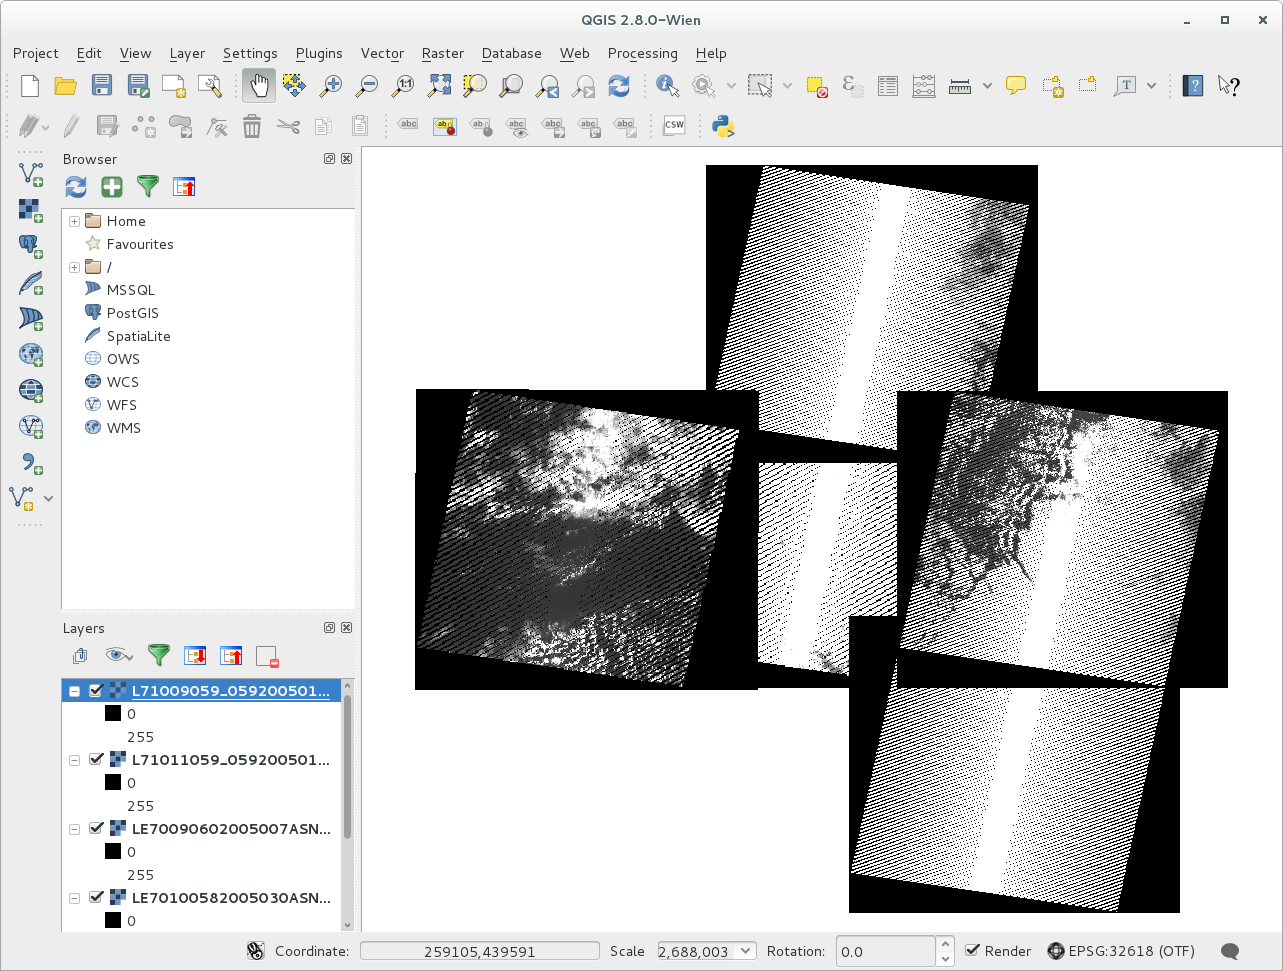
\includegraphics[width=12cm]{pictures/bio1.png}
  \caption{Imágenes Landsat de Nariño}
  \label{fig:bio1}
\end{figure}


\section{Reproyectar y recortar imágenes satelitales}

Debido a que las imágenes satelitales que cubren el departamento de Nariño, no estan en el mismo sistema de coordenadas, se tubo que hacer
una transformación de todas las imágenes a un mismo sistema de coordenadas, que además este sistema se pueda trabajar en metros decimales,
por lo tanto el sistema al cual se transformo fue al sistema EPSG:3857.

También debido a que las imágenes para el departamento de Nariño, sobrepasan mucho más el área del departamento, se recortó las imágenes
haciendo un buffer de 2500 metros de un shapfile del departamento y sobre este se extrajo el área del departamento, de esta manera los datos 
que se capturen únicamente corresponderan al departamento de Nariño, como lo muestra la figura~\ref{fig:bio2}

\begin{figure}[!htb]
  \centering
  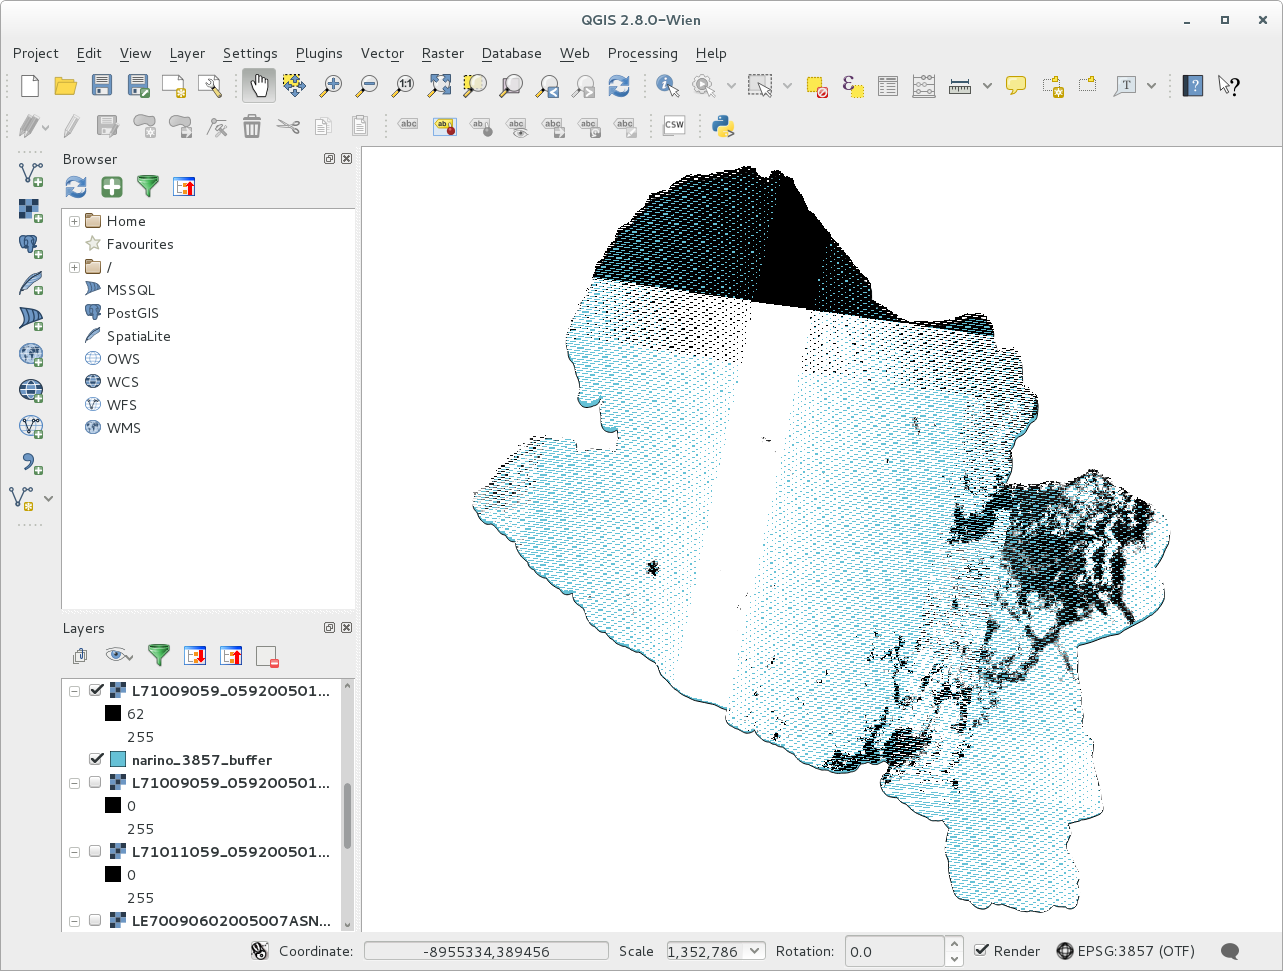
\includegraphics[width=12cm]{pictures/bio2.png}
  \caption{Imágenes Landsat de Nariño recortadas}
  \label{fig:bio2}
\end{figure}

Este proceso se aplico a las 1362 imágenes, para esto se lo realizo utilizando un script el cual se encuentra en repositorio del proyecto
\footnote{\url{https://github.com/poldrosky/alternar.git}}.


\section{Diseño de base de datos}

Se diseña una base de datos la cual va a guardar la información contenida en las imágenes satelitales, recorriendolas pixel a pixel. El diseño se lo puede mirar
en la figura~\ref{fig:dise}

\begin{figure}[!htb]
  \centering
  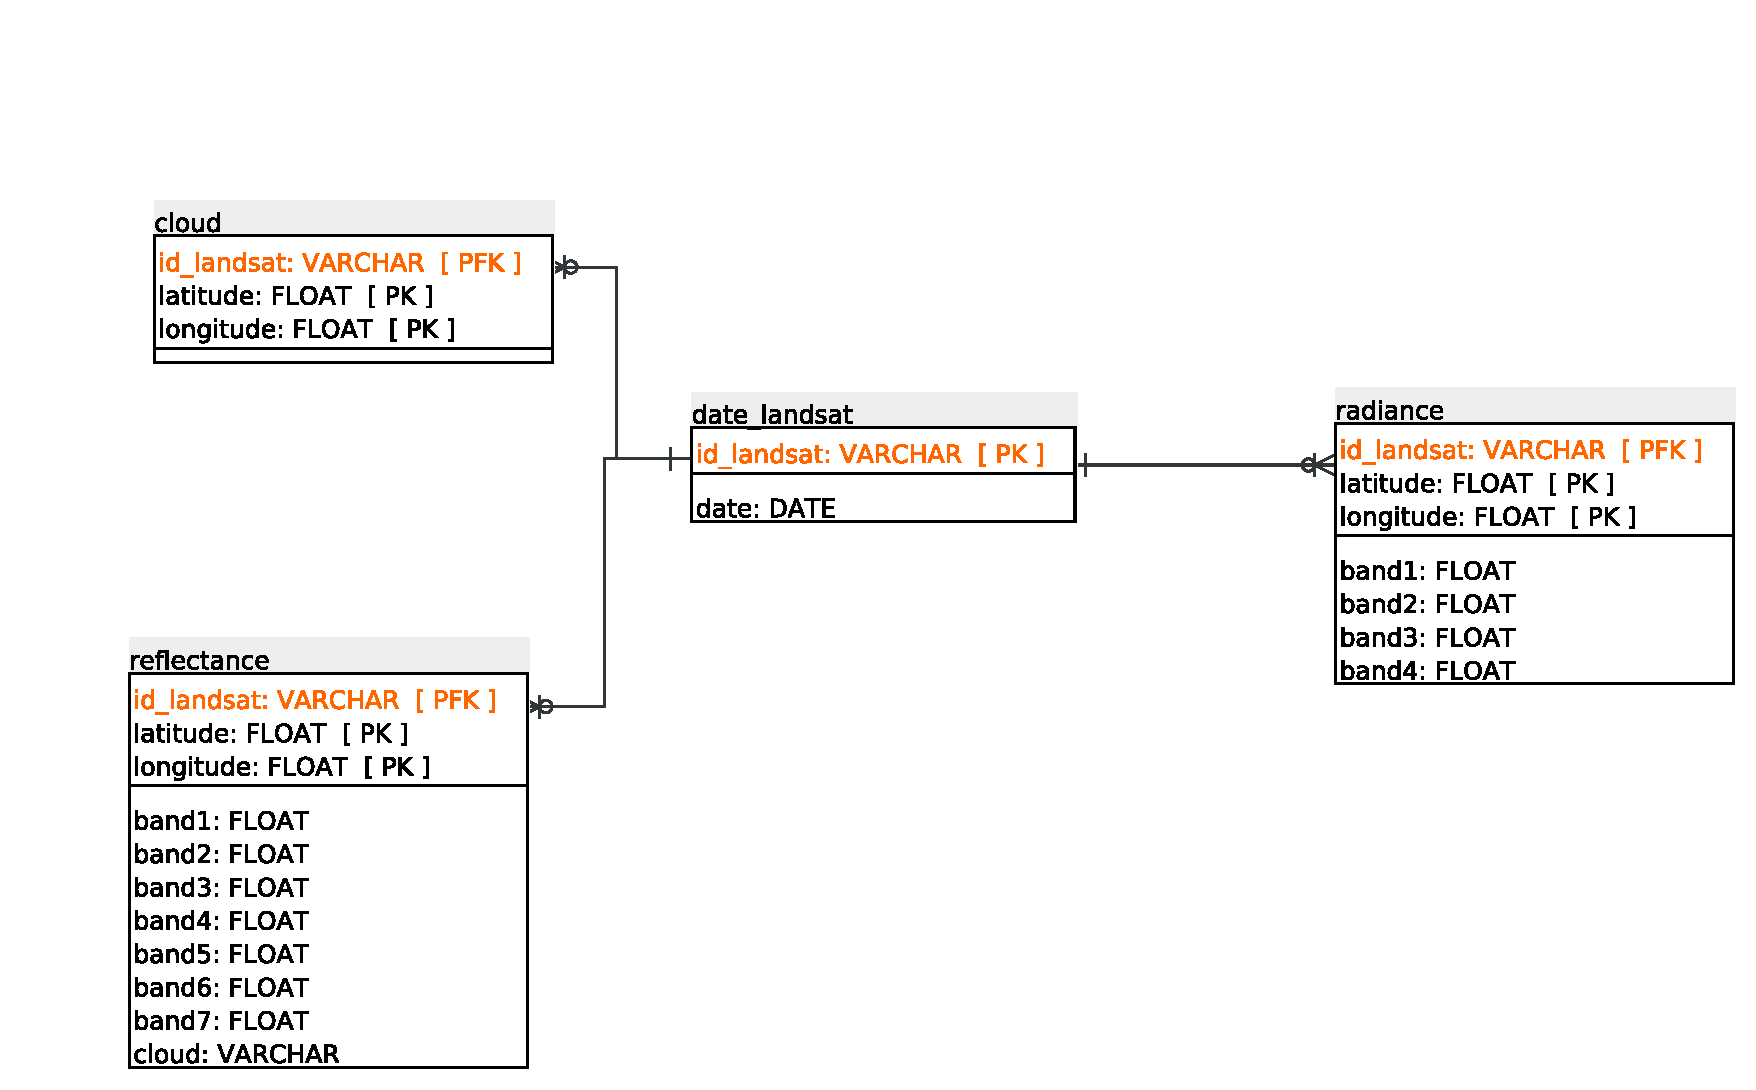
\includegraphics[width=12cm]{pictures/diagramaER.pdf}
  \caption{Diagrama ER de la Base de datos}
  \label{fig:dise}
\end{figure}


\section{Captura de información}

En la captura de información se tienen varios aspectos, como calculo de radiance, reflectance, y además se aplico un 
algoritmo propuesto en \cite{irish2000landsat}, en el cual se realiza un filtro para la detección de nubes.

Para la realización de este proceso se realizó un scrip que se encuentra en el repositorio del proyecto.


